\chapter{Introdução}

\section{Objetivos}

\section{Justificativa}

\section{Metodologia de trabalho}

A pesquisa consiste em propor um processo que auxilie na refatoração de arquitetura em projetos de software que utilizam métodos ágeis.

O plano de pesquisa a ser utilizado seguirá orientações de \cite{dias2010developing} através uma abordagem baseada em evidências, esta inclui as seguintes atividades principais:
\begin{enumerate}[(a)]

\item Identificar estudos preliminares: condução de revisão sistemática da literatura com a finalidade de identificar estudos relacionados a refatoração de arquitetura nos métodos ágeis, que tratem de métodos ou práticas utilizados e problemas vivenciados.

\item Proposta da abordagem: proposta de uma abordagem para auxiliar na atividade de refatoração de arquiteturas nos métodos ágeis: definição de atividades a serem desenvolvidas, processo a ser seguido e recomendações de forma de adequação aos princípios ágeis. A proposta será construída baseada nas evidências.

\item Validação da proposta com especialista: Considerando que a proposta apresenta tanto contribuições práticas quanto teórica, a validação da proposta será realizada com especialista da academia e profissionais da indústria. Como representantes da academia serão entrevistados 2 pesquisadores da área de Engenharia de Software e como representantes da indústria serão entrevistados 2 consultores sobre métodos ágeis. Para realização da validação será utilizada a técnica de grupos focados. O planejamento das reuniões, a condução das reuniões e forma de análise dos dados, seguirão as recomendações de \cite{ribeiro2003gruposfocados}.

\item Validação da proposta através da aplicação em uma situação real: realização de uma pesquisa-ação numa empresa que apresenta o contexto de pesquisa estudado. Para realização da pesquisa-ação serão seguidas as recomendações de \cite{dos2008colaboraccao}. As métricas utilizadas para a validação durante o processo de pesquisa-ação serão levantadas com base no acompanhamento de \textit{sprints} realizadas pelo desenvolvimento da empresa, sendo considerados para este levantamento os seguintes relatórios:
    
   \begin{itemize}
        \item Diagrama acumulativo de fluxo de tarefas.
        \item Gráfico de controle para medição de estabilidade de métricas.
        \item Gráfico de velocidade para histórias implementadas.
        \item Gráfico burndown para apresentação de alterações de escopo não planejado.
    \end{itemize}  
    
\end{enumerate}

As validações à serem aplicadas utilizam métricas que já são monitoradas atualmente no ambiente de desenvolvimento da empresa em questão onde a pesquisa-ação será realizada, desta maneira será possível avaliar com maior embasamento o impacto que a aplicação da melhoria proposta tratá ao ambiente de desenvolvimento e consequentemente às métricas de acompanhamento. A figura \ref{fig:estrategia_pesquisa} apresenta a metodologia de pesquisa proposta, que inclui as seguintes atividades principais:
\begin{figure}[ht]
\centering
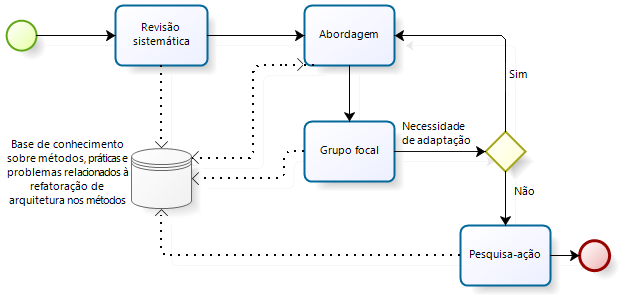
\includegraphics[scale=0.90]{figuras/estrategia_pesquisa}
\caption{ Estratégia de pesquisa}
% \resizebox{!}{0.3cm}{}
\label{fig:estrategia_pesquisa}
\end{figure}



% \subsection{Resultados esperados}

% De acordo com \cite{kitchenham2004evidence} os papeis atuantes na gestão de desenvolvimento de software constantemente são questionados sobre qual a efetividade do investimento em determinadas tecnologias e o seu retorno após a implantação da mesma. A pesquisa-ação de tecnologias e técnicas permitem manter um nível razoável de segurança refinando estas técnicas em meios acadêmicos antes de disponibilizá-las à indústria \cite{dias2010developing}. 

% Através da apresentação da proposta e da pesquisa-ação à ser realizada, busca-se compreender a aplicação da refatoração de produtos de software com métodos ágeis aplicados pela indústria ligados aos objetivos de qualidade esperados. Neste contexto espera-se apresentar uma proposta de melhoria no processo de refatoração de arquiteturas de software auxiliando-as à atingir uma arquitetura de produto satisfatória em concordância com a flexibilidade proporcionada pelos métodos ágeis. 